\section{Staff Usage}
\label{sec:staff_usage}
The \astaff[] members main usage of the is to solve problems.
This is corresponding to the \ucsolproblem{} use case in section \ref{sec:usecase}.
This use case is how ever quite large, so it is divided into three steps; choosing a problem to solve, communicate with the subscriber(s), solve the problem.
The communication with the subscriber(s) step might not be applied during the solve usage of the \aclient[].
The three steps are described in the following subsections.

\subsection{Choosing a Problem to Solve}
\begin{figure}[htb]
	\centering
		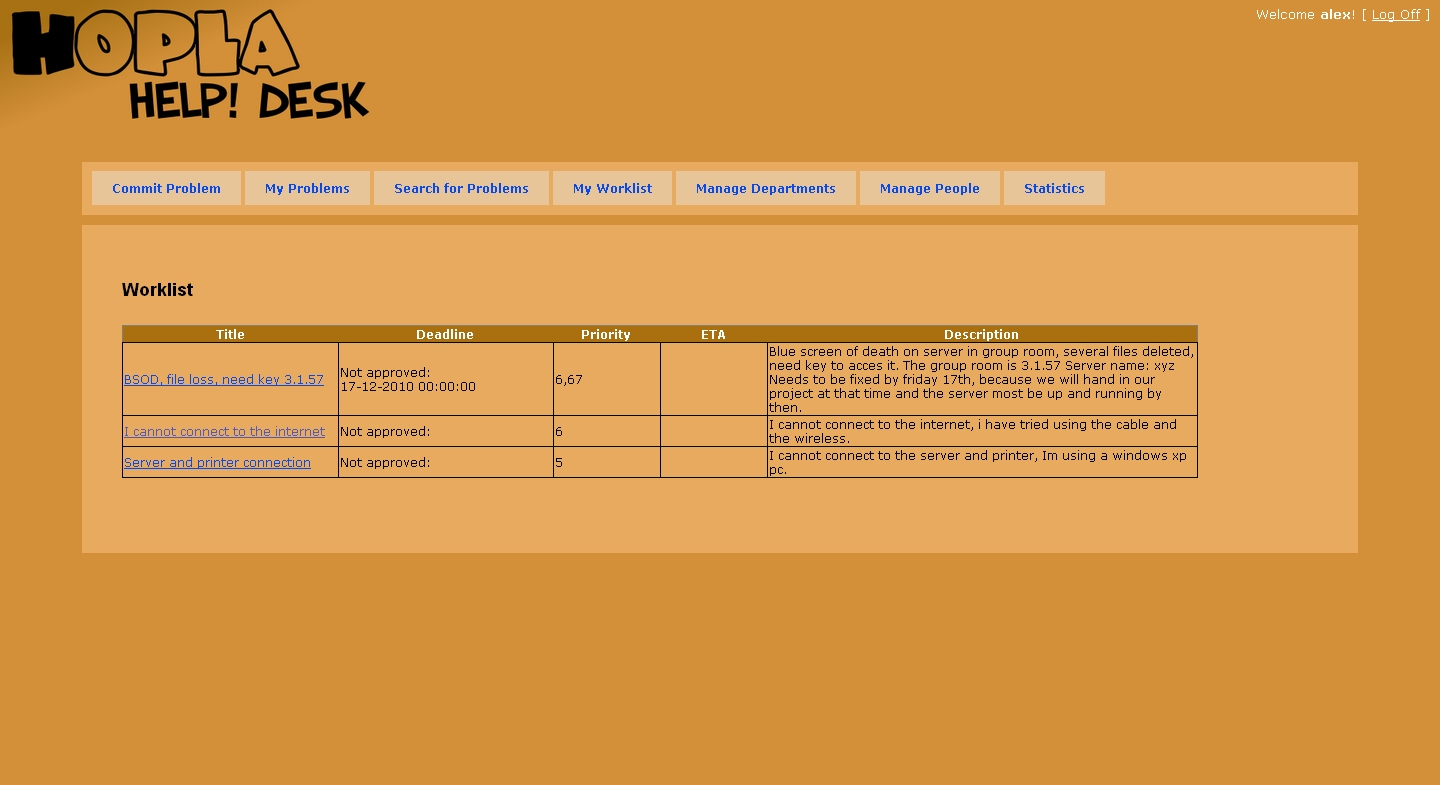
\includegraphics[width=1.00\textwidth, clip=true, trim=4cm 10.5cm 8cm 8cm]{input/implementation/program_presentation/worklist.png}
	\morscaption{A \astaff[] members worklist}
	\label{fig:worklist}
\end{figure}

When a \astaff[] member wants to solve a problem he/she clicks the menu point called My Worklist which can be seen in figure \ref{fig:master}.
This shows the worklist of current logged in \astaff[] user.
An example of a worklist is shown in figure \ref{fig:worklist}.
The \astaff[] member can see the title, description, deadline, priority, and ETC

\subsection{Communicate With Subscribers}


\subsection{Solve the Problem}